\section{Trigonometric Substitution}\label{sec:trig_sub}

In Section \ref{sec:def_int} we defined the definite integral as the ``signed area under the curve.'' In that section we had not yet learned the Fundamental Theorem of Calculus, so we evaluated special definite integrals which described nice, geometric shapes. For instance, we were able to evaluate
\begin{equation}
\int_{-3}^3\sqrt{9-x^2}\ dx = \frac{9\pi}{2}\label{eq:trigsub1}
\end{equation}
 as we recognized that $f(x) = \sqrt{9-x^2}$ described the upper half of a circle with radius 3. 

We have since learned a number of integration techniques, including Substitution and Integration by Parts, yet we are still unable to evaluate the above integral without resorting to a geometric interpretation. This section introduces Trigonometric Substitution, a method of integration that fills this gap in our integration skill. This technique works on the same principle as Substitution as found in Section \ref{sec:substitution}, though it can feel ``backward.'' In Section \ref{sec:substitution}, we set $u=f(x)$, for some function $f$, and replaced $f(x)$ with $u$. In this section, we will set $x=f(\theta)$, where $f$ is a trigonometric function, then replace $x$ with $f(\theta)$. 

We start by demonstrating this method in evaluating the integral in \eqref{eq:trigsub1}. After the example, we will generalize the method and give more examples.\\
\enlargethispage{3\baselineskip}

\example{ex_trigsub1}{Using Trigonometric Substitution}{
Evaluate $\ds \int_{-3}^3\sqrt{9-x^2}\ dx$.}
{We begin by noting that $9\sin^2\theta + 9\cos^2\theta = 9$, and hence $9\cos^2\theta = 9-9\sin^2\theta$. If we let $x=3\sin\theta$, then $9-x^2 = 9-9\sin^2\theta = 9\cos^2\theta$. 

Setting $x=3\sin \theta$ gives  $dx = 3\cos\theta\ d\theta$. We are almost ready to substitute. We also wish to change our bounds of integration. The bound $x=-3$ corresponds to $\theta = -\pi/2$ (for when $\theta = -\pi/2$, $x=3\sin \theta = -3$). Likewise, the bound of $x=3$ is replaced by the bound $\theta = \pi/2$. Thus
\begin{align*}
\int_{-3}^3\sqrt{9-x^2}\ dx &= \int_{-\pi/2}^{\pi/2} \sqrt{9-9\sin^2\theta} (3\cos\theta)\ d\theta \\
		&= \int_{-\pi/2}^{\pi/2} 3\sqrt{9\cos^2\theta} \cos\theta\ d\theta \\
		&=\int_{-\pi/2}^{\pi/2} 3|3\cos \theta| \cos\theta\ d\theta.
		\intertext{On $[-\pi/2,\pi/2]$, $\cos \theta$ is always positive, so we can drop the absolute value bars, then employ a power--reducing formula:}
\end{align*}
\begin{align*}
			&= \int_{-\pi/2}^{\pi/2} 9\cos^2 \theta\ d\theta\\
			&= \int_{-\pi/2}^{\pi/2} \frac{9}{2}\big(1+\cos(2\theta)\big)\ d\theta\\
			& = \frac92 \big(\theta +\frac12\sin(2\theta)\big)\Bigg|_{-\pi/2}^{\pi/2}= \frac92\pi.
\end{align*}
This matches our answer from before.
}\\

We now describe in detail Trigonometric Substitution. This method excels when dealing with integrands that contain $\sqrt{a^2-x^2}$, $\sqrt{x^2-a^2}$ and $\sqrt{x^2+a^2}$. The following Key Idea outlines the procedure for each case, followed by more examples. Each right triangle acts as a reference to help us understand the relationships between $x$ and $\theta$.
\enlargethispage{2\baselineskip}

\setboxwidth{100pt}
\hskip-100pt%
\noindent\begin{minipage}{\linewidth+100pt}
\keyidea{idea:trigsub}{Trigonometric Substitution}
{For the three cases below, we assume that $a>0$.
\begin{enumerate}
	\item[(a)] \noindent%
		\begin{minipage}[t]{.6\linewidth}%
		For integrands containing $\sqrt{a^2-x^2}$:\index{integration!trig. subst.}\\[5pt]
		Let $x=a\sin\theta$, \qquad $dx = a\cos\theta\ d\theta$\\[5pt]	
	Thus $\theta = \sin^{-1}(x/a)$, for $-\pi/2\leq \theta\leq \pi/2$. \\[5pt]	
	On this interval, $\cos\theta\geq 0$, so\\[5pt]	
	$\sqrt{a^2-x^2} = a\cos\theta$
		\end{minipage}\qquad
	\begin{minipage}[t]{.4\linewidth}\vskip 0pt
		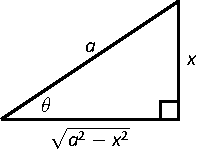
\includegraphics{figures/figtrigsub_intro1}
		\end{minipage}
		
	\item[(b)] \noindent
	\begin{minipage}[t]{.6\linewidth}
		For integrands containing $\sqrt{x^2+a^2}$:\\[5pt]
		Let $x=a\tan\theta$, \qquad $dx = a\sec^2\theta\ d\theta$\\[5pt]	
	Thus $\theta = \tan^{-1}(x/a)$, for $-\pi/2 < \theta < \pi/2$. \\[5pt]	
	On this interval, $\sec\theta> 0$, so\\[5pt]	
	$\sqrt{x^2+a^2} = a\sec\theta$
		\end{minipage}\qquad
	\begin{minipage}[t]{.4\linewidth}\vskip 0pt
		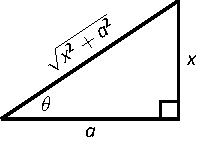
\includegraphics{figures/figtrigsub_intro3}
		\end{minipage}
		
	\item[(c)] \noindent
	\begin{minipage}[t]{.6\linewidth}
		For integrands containing $\sqrt{x^2-a^2}$:\\[5pt]
		Let $x=a\sec\theta$, \qquad $dx = a\sec\theta\tan\theta\ d\theta$\\[5pt]	
	Thus $\theta = \sec^{-1}(x/a)$. Note that $\sqrt{x^2-a^2}$ is defined for $x\geq a$ or $x\leq -a$.\\
	 If $x\geq a$, then $x/a\geq 1$ and $0\leq\theta<\pi/2$; if $x<-a$, then $x/a \leq -1$ and $\pi\leq\theta< \frac{3\pi}{2}$.\\[5pt]	
	On these intervals, $\tan\theta\geq 0$, so\\[5pt]	
	$\sqrt{x^2-a^2} = a\tan\theta$
		\end{minipage}\qquad
	\begin{minipage}[t]{.4\linewidth}\vskip 0pt
		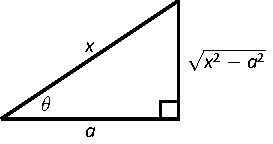
\includegraphics{figures/figtrigsub_intro2}
		\end{minipage}	
\end{enumerate}
}
\end{minipage}
\restoreboxwidth
\vskip \baselineskip

\example{ex_trigsub3}{Using Trigonometric Substitution}{
Evaluate $\ds \int \frac{1}{\sqrt{5+x^2}}\ dx.$}
{Using Key Idea \ref{idea:trigsub}(b), we recognize $a=\sqrt{5}$ and  set $x= \sqrt{5}\tan \theta$. This makes $dx = \sqrt{5}\sec^2\theta\ d\theta$. We will use the fact that $\sqrt{5+x^2} = \sqrt{5+5\tan^2\theta} = \sqrt{5\sec^2\theta} = \sqrt{5}\sec\theta.$ Substituting, we have:
\begin{align*}
\int \frac{1}{\sqrt{5+x^2}}\ dx &= \int \frac{1}{\sqrt{5+5\tan^2\theta}}\sqrt{5}\sec^2\theta\ d\theta \\
			&= \int \frac{\sqrt{5}\sec^2\theta}{\sqrt{5}\sec\theta} \ d\theta\\
			&= \int \sec\theta\ d\theta\\
			&= \ln\big|\sec\theta+\tan\theta\big|+C.
\end{align*}
While the integration steps are over, we are not yet done. The original problem was stated in terms of $x$, whereas our answer is given in terms of $\theta$. We must convert back to $x$.

The reference triangle given in Key Idea \ref{idea:trigsub}(b) helps. With $x=\sqrt{5}\tan\theta$, we have 
\[
\tan \theta = \frac x{\sqrt{5}}\quad \text{and}\quad \sec\theta = \frac{\sqrt{x^2+5}}{\sqrt{5}}.
\]
This gives
\begin{align*}
\int \frac{1}{\sqrt{5+x^2}}\ dx &= \ln\big|\sec\theta+\tan\theta\big|+C \\
     &= \ln\left|\frac{\sqrt{x^2+5}}{\sqrt{5}}+ \frac x{\sqrt{5}}\right|+C.
\end{align*}
We can leave this answer as is, or we can use a logarithmic identity to simplify it. Note:
\begin{align*}
\ln\left|\frac{\sqrt{x^2+5}}{\sqrt{5}}+ \frac x{\sqrt{5}}\right|+C &= \ln\left|\frac{1}{\sqrt{5}}\big(\sqrt{x^2+5}+ x\big)\right|+C \\
   &= \ln\left|\frac{1}{\sqrt{5}}\right| + \ln\big|\sqrt{x^2+5}+ x\big|+C\\
	&=	\ln\big|\sqrt{x^2+5}+ x\big|+C,
\end{align*}
where the $\ln\big(1/\sqrt{5}\big)$ term is absorbed into the constant $C$. (In Section \ref{sec:hyperbolic} we will learn another way of approaching this problem.)
}\\

\example{ex_trigsub2}{Using Trigonometric Substitution}{
Evaluate $\ds \int \sqrt{4x^2-1}\ dx$.}
{We start by rewriting the integrand so that it looks like $\sqrt{x^2-a^2}$ for some value of $a$:
\begin{align*}
\sqrt{4x^2-1} &= \sqrt{4\left(x^2-\frac14\right)}\\
		&= 2\sqrt{x^2-\left(\frac12\right)^2}.
\end{align*}
So we have $a=1/2$, and following Key Idea \ref{idea:trigsub}(c), we set $x= \frac12\sec\theta$, and hence $dx = \frac12\sec\theta\tan\theta\ d\theta$. %The Key Idea also shows that $\sqrt{x^2-1/2^2} = \frac12\tan\theta$. 
We now rewrite the integral with these substitutions:
\begin{align*}
\int \sqrt{4x^2-1}\ dx &= \int 2\sqrt{x^2-\left(\frac12\right)^2}\ dx\\
			&= \int 2\sqrt{\frac14\sec^2\theta - \frac14}\left(\frac12\sec\theta\tan\theta\right)\ d\theta\\
			&=\int \sqrt{\frac14(\sec^2\theta-1)}\Big(\sec\theta\tan\theta\Big)\ d\theta\\
			&=\int\sqrt{\frac14\tan^2\theta}\Big(\sec\theta\tan\theta\Big)\ d\theta\\
			&=\int \frac12\tan^2\theta\sec\theta\ d\theta\\
			&=\frac12\int \Big(\sec^2\theta-1\Big)\sec\theta\ d\theta\\
			&=\frac12\int \big(\sec^3\theta - \sec\theta\big)\ d\theta.
\end{align*}
We integrated $\sec^3\theta$ in Example \ref{ex_trigint6}, finding its antiderivatives to be
\[
\int \sec^3\theta\ d\theta = \frac12\Big(\sec \theta\tan \theta + \ln|\sec \theta+\tan \theta|\Big)+C.
\]
\enlargethispage{2\baselineskip}
Thus
\begin{align*}
\int \sqrt{4x^2-1}\ dx &=\frac12\int \big(\sec^3\theta - \sec\theta\big)\ d\theta\\
			&= \frac12\left(\frac12\Big(\sec \theta\tan \theta + \ln|\sec \theta+\tan \theta|\Big) -\ln|\sec \theta + \tan\theta|\right) + C\\
			%\end{align*}
			%\begin{align*}
			&= \frac14\left(\sec\theta\tan\theta -\ln|\sec\theta+\tan\theta|\right)+C.
\end{align*}
We are not yet done. Our original integral is given in terms of $x$, whereas our final answer, as given, is in terms of $\theta$. We need to rewrite our answer in terms of $x$. With $a=1/2$, and $x=\frac12\sec\theta$, the reference triangle in Key Idea \ref{idea:trigsub}(c) shows that 
\[
\tan \theta = \sqrt{x^2-1/4}\Big/(1/2) = 2\sqrt{x^2-1/4}\quad \text{and}\quad \sec\theta = 2x.
\]
Thus\small 
\begin{align*}
\frac14\Big(\sec\theta\tan\theta -\ln\big|\sec\theta+\tan\theta\big|\Big)+C &=
				\frac14\Big(2x\cdot 2\sqrt{x^2-1/4} - \ln\big|2x + 2\sqrt{x^2-1/4}\big|\Big)+C\\
				&= \frac14\Big(4x\sqrt{x^2-1/4} - \ln\big|2x + 2\sqrt{x^2-1/4}\big|\Big)+C.
\end{align*}
\normalsize 
The final answer is given in the last line above, repeated here:
\[
\int \sqrt{4x^2-1}\ dx = \frac14\Big(4x\sqrt{x^2-1/4} - \ln\big|2x + 2\sqrt{x^2-1/4}\big|\Big)+C.
\]
}\\

\example{ex_trigsub4}{Using Trigonometric Substitution}{
Evaluate $\ds \int \frac{\sqrt{4-x^2}}{x^2}\ dx$.}
{We use Key Idea \ref{idea:trigsub}(a) with $a=2$, $x=2\sin \theta$, $dx = 2\cos \theta$ and hence $\sqrt{4-x^2} = 2\cos\theta$. This gives
\begin{align*}
\int \frac{\sqrt{4-x^2}}{x^2}\ dx &= \int \frac{2\cos\theta}{4\sin^2\theta}(2\cos\theta)\ d\theta\\
		&= \int \cot^2\theta\ d\theta\\
		&=	\int (\csc^2\theta -1)\ d\theta\\
		&= -\cot\theta -\theta + C.
\end{align*}
We need to rewrite our answer in terms of $x$. Using the reference triangle found in Key Idea \ref{idea:trigsub}(a), we have $\cot\theta = \sqrt{4-x^2}/x$ and $\theta = \sin^{-1}(x/2)$. Thus
\[
\int \frac{\sqrt{4-x^2}}{x^2}\ dx = -\frac{\sqrt{4-x^2}}x-\sin^{-1}\left(\frac x2\right) + C.
\]
}\\

Trigonometric Substitution can be applied in many situations, even those not of the form $\sqrt{a^2-x^2}$, $\sqrt{x^2-a^2}$ or $\sqrt{x^2+a^2}$. In the following example, we apply it to an integral we already know how to handle.\\

\example{ex_trigsub5}{Using Trigonometric Substitution}{
Evaluate $\ds \int\frac1{x^2+1}\ dx$.}
{We know the answer already as $\tan^{-1}x+C$. We apply Trigonometric Substitution here to show that we get the same answer without inherently relying on knowledge of the derivative of the arctangent function.

Using Key Idea \ref{idea:trigsub}(b), let $x=\tan\theta$, $dx=\sec^2\theta\ d\theta$ and note that $x^2+1 = \tan^2\theta+1 = \sec^2\theta$. Thus
\begin{align*}
\int \frac1{x^2+1}\ dx &= \int \frac{1}{\sec^2\theta}\sec^2\theta\ d\theta \\
			&= \int 1\ d\theta\\
			&= \theta + C.
\end{align*}
Since $x=\tan \theta$, $\theta = \tan^{-1}x$, and we conclude that $\ds \int\frac1{x^2+1}\ dx = \tan^{-1}x+C.$
}\\

The next example is similar to the previous one in that it does not involve a square--root. It shows how several techniques and identities can be combined to obtain a solution.\\

\example{ex_trigsub7}{Using Trigonometric Substitution}{
Evaluate $\ds\int\frac1{(x^2+6x+10)^2}\ dx.$
}
{We start by completing the square, then make the substitution $u=x+3$, followed by the trigonometric substitution of $u=\tan\theta$:
\begin{align}
\int \frac1{(x^2+6x+10)^2}\ dx =\int \frac1{\big((x+3)^2+1\big)^2}\ dx&= \int \frac1{(u^2+1)^2}\ du. \notag
\intertext{Now make the substitution $u=\tan\theta$, $du=\sec^2\theta\ d\theta$:}
   &=	\int \frac1{(\tan^2\theta+1)^2}\sec^2\theta\ d\theta\notag\\
	&= \int\frac 1{(\sec^2\theta)^2}\sec^2\theta\ d\theta\notag\\
	&= \int \cos^2\theta\ d\theta.\notag
	\intertext{Applying a power reducing formula, we have}
	&= \int \left(\frac12 +\frac12\cos(2\theta)\right)\ d\theta \notag\\
	&= \frac12\theta + \frac14\sin(2\theta) + C.\label{eq:extrigsub7}
\end{align}
We need to return to the variable $x$. As $u=\tan\theta$, $\theta = \tan^{-1}u$. Using the identity $\sin(2\theta) = 2\sin\theta\cos\theta$ and using the reference triangle found in Key Idea \ref{idea:trigsub}(b), we have 
\[
\frac14\sin(2\theta) = \frac12\frac u{\sqrt{u^2+1}}\cdot\frac 1{\sqrt{u^2+1}} = \frac12\frac u{u^2+1}.
\]
Finally, we return to $x$ with the substitution $u=x+3$. We start with the expression in Equation \eqref{eq:extrigsub7}:
\begin{align*}
\frac12\theta + \frac14\sin(2\theta) + C &= \frac12\tan^{-1}u + \frac12\frac{u}{u^2+1}+C\\
				&= \frac12\tan^{-1}(x+3) + \frac{x+3}{2(x^2+6x+10)}+C.
\end{align*}
Stating our final result in one line,
\[
\int\frac1{(x^2+6x+10)^2}\ dx=\frac12\tan^{-1}(x+3) + \frac{x+3}{2(x^2+6x+10)}+C.
\]
}\\


Our last example returns us to definite integrals, as seen in our first example. Given a definite integral that can be evaluated using Trigonometric Substitution, we could first evaluate the corresponding indefinite integral (by changing from an integral in terms of $x$ to one in terms of $\theta$, then converting back to $x$) and then evaluate using the original bounds. It is much more straightforward, though, to change the bounds as we substitute.\\

\example{ex_trigsub6}{Definite integration and Trigonometric Substitution}{
Evaluate $\ds\int_0^5\frac{x^2}{\sqrt{x^2+25}}\ dx$.
}
{Using Key Idea \ref{idea:trigsub}(b), we set $x=5\tan\theta$, $dx = 5\sec^2\theta\ d\theta$, and note that $\sqrt{x^2+25} = 5\sec\theta$. As we substitute, we can also change the bounds of integration.

The lower bound of the original integral is $x=0$. As $x=5\tan\theta$, we solve for $\theta$ and find $\theta = \tan^{-1}(x/5)$. Thus the new lower bound is $\theta = \tan^{-1}(0) = 0$. The original upper bound is $x=5$, thus the new upper bound is $\theta = \tan^{-1}(5/5) = \pi/4$. 

Thus we have 
\begin{align*}
\int_0^5\frac{x^2}{\sqrt{x^2+25}}\ dx &= \int_0^{\pi/4} \frac{25\tan^2\theta}{5\sec\theta}5\sec^2\theta\ d\theta\\
		&= 25\int_0^{\pi/4} \tan^2\theta\sec\theta\ d\theta.
\end{align*}
We encountered this indefinite integral in Example \ref{ex_trigsub2} where we found 
\[
\int \tan^2\theta\sec\theta \ d\theta = \frac12\big(\sec\theta\tan\theta-\ln|\sec\theta+\tan\theta|\big).
\]
So
\begin{align*}
25\int_0^{\pi/4} \tan^2\theta\sec\theta\ d\theta &= \frac{25}2\big(\sec\theta\tan\theta-\ln|\sec\theta+\tan\theta|\big)\Bigg|_0^{\pi/4}\\
&= \frac{25}2\big(\sqrt2-\ln(\sqrt2+1)\big)\\
&\approx 6.661.
\end{align*}
\vskip-1.5\baselineskip
}\\

\enlargethispage{3\baselineskip}
The following equalities are very useful when evaluating integrals using Trigonometric Substitution. 

\keyidea{idea:useful_trigsub}{Useful Equalities with Trigonometric Substitution}
{\begin{enumerate}
	\item	$\sin(2\theta) = 2\sin\theta\cos\theta$
	\item	$\cos(2\theta) = \cos^2\theta - \sin^2\theta = 2\cos^2\theta-1 = 1-2\sin^2\theta$
	\item $\ds \int \sec^3\theta\ d\theta = \frac12\Big(\sec \theta\tan \theta + \ln\big|\sec \theta+\tan \theta\big|\Big)+C$
	\item	$\ds \int \cos^2\theta\ d\theta = \int \frac12\big(1+\cos(2\theta)\big)\ d\theta = \frac12\big(\theta+\sin\theta\cos\theta\big)+C.$
\end{enumerate}
}

%\subsection*{Hyperbolic substitution}
%For integrands containing terms of the form $\sqrt{x^2+a^2}$ or $\sqrt{x^2-a^2}$, it is also possible to make use of \sword{hyperbolic substitution} \index{substitution ! hyperbolic}. Recall from Section \ref{sec:hyperbolic} of the Math 1560 textbook that the hyperbolic functions are defined by
%\[
%\cosh(x) = \frac{e^x+e^{-x}}{2} \quad \text{ and } \quad \sinh(x) %= \frac{e^x-e^{-x}}{2},
%\]
%with $\tanh(x) = \dfrac{\sinh(x)}{\cosh(x)}$, and so on. Recall that the hyperbolic functions satisfy the identity
%\[
%\cosh^2(x)-\sinh^2(x)  = 1.
%\]
%If we're given $\sqrt{x^2+a^2}$, we can let $x=a\sinh(t)$, then
%\[
%x^2+a^2 = (a\sinh(t))^2+a^2 = a^2(\sinh^2(t)+1) = a^2\cosh^2(t),
%\]
%and $dx = a\cosh(t)\,dt$. Since $\cosh(t)>0$ for all real numbers $t$, we have $\sqrt{a^2+x^2}=\cosh(t)$.

%If we're given $\sqrt{x^2-a^2}$, we can let $x=a\cosh(t)$; then
%\[
%x^2-a^2 = (a\cosh(t))^2-a^2 = a^2(\cosh^2(t)-1) = a^2\sinh^2(t),
%\]
%and $dx = a\sinh(t)$. (One of the convenient aspects of working with hyperbolic functions is that there are no signs to worry about when taking derivatives.)
%Note that $\cosh(t)>0$ for all $t$, so the substitution $x=a\cosh(t)$ works in the case that $x\geq a>0$. In this case, $\sqrt{x^2-a^2} = a\sinh(t)$. For $x<-a<0$, technically we would need to let $x=-a\cosh(t)$. We illustrate this method with a couple of examples.\\

%\example{ex_hypsub1}{Using hyperbolic substitution}{
%Use hyperbolic substitution to evaluate the integral $\displaystyle \int\frac{3}{\sqrt{x^2+4}}\,dx$.
%}
%{
%Here we encounter the form $\sqrt{x^2+4} = \sqrt{x^2+2^2}$, so we use the substitution $x=2\sinh(t)$, or $t=\sinh^{-1}(x/2)$. This gives us
%\[
%\sqrt{x^2+4} = \sqrt{4\sinh^2(t)+4} = \sqrt{4\cosh^2(t)}=2\cosh(t),
%\]
%and $dx = 4\cosh(t)\,dt$. Substituting these into the integral, we have
%\begin{align*}
%\int\frac{3}{\sqrt{x^2+4}}\,dx &= \int \frac{3(2\cosh(t))}{2\cosh(t)}\,dt\\
%& = \int 3 \,dt = 3t+C\\
%& = 3\sinh^{-1}\left(\frac{x}{2}\right)+C.
%\end{align*}

%Of course, we could also evaluate the integral using the substitution $x=2\tan\theta$. In this case, the hyperbolic substitution turns out to be much simpler. Let's go through the details to confirm this. If $x=2\tan\theta$, then we have $dx = 2\sec^2\theta\,d\theta$, and
%\[
%\sqrt{x^2+4} = \sqrt{4\tan^2\theta+4} = \sqrt{4\sec^2\theta} = 2\sec\theta.
%\]
%In terms of $\theta$, our integral is
%\begin{align*}
%\int\frac{3}{\sqrt{x^2+4}}\,dx & = \int \frac{3(2\sec^2\theta)}{2\sec\theta}\,d\theta\\
% & = \int 3\sec\theta\,d\theta\\
% & = 3\ln\lvert \sec\theta +\tan\theta\rvert+C\\
% & = 3\ln\left( \frac{\sqrt{x^2+4}}{2} + \frac{x}{2}\right) +C.
%\end{align*}
%(Note that since $\sqrt{x^2+4}>x$ for all values of $x$, we can drop the absolute value in the argument of the logarithm.)

%The answer using the hyperbolic substitution certainly looks simpler, and it was easier to obtain, but are the two results equivalent? That is, is it true that
%\[
%\sinh^{-1}\left(\frac{x}{2}\right) = \ln\left(\frac{\sqrt{x^2+4}+x}{2}\right)?
%\]
%To check, let's take the hyperbolic sine of both sides. On the left, this yields $\frac{x}{2}$. On the right, we get
%\begin{align*}
%\sinh\left[\ln\left(\frac{\sqrt{x^2+4}+x}{2}\right)\right] & = \frac{1}{2}\left[e^{\ln\left(\frac{\sqrt{x^2+4}+x}{2}\right)}-e^{\ln\left(\frac{\sqrt{x^2+4}+x}{2}\right)}\right]\\
%& = \frac{1}{2}\left[\frac{\sqrt{x^2+4}+x}{2}-\frac{2}{\sqrt{x^2+4}+x}\right]\\
%& = \frac{1}{2}\left[\frac{(\sqrt{x^2+4}+x)^2-4}{2(\sqrt{x^2+4}+x)}\right]\\
%& = \frac{1}{4}\left[\frac{(x^2+4)+2x\sqrt{x^2+4}+x^2-4}{\sqrt{x^2+4}+x}\right]\\
%& = \frac{1}{4}\left[\frac{2x(\sqrt{x^2+4}+x)}{\sqrt{x^2+4}+x}\right]\\
%& = \frac{x}{2},
%\end{align*}
%so the results agree!
%}\\

%\example{ex_hypsub2}{Using hyperbolic substitution}{
%Evaluate the integral $\displaystyle \int\frac{x^2}{\sqrt{x^2-16}}\,dx$ using a hyperbolic substitution.
%}
%{Once again, we \textit{could} use the substitution $x=4\sec\theta$, but doing so leads us to a $\sec^3\theta$ integral, and those are never fun. (Feel free to try it this way) Instead, we decide to read (and follow) the instructions, and use a hyperbolic substitution.

%The form $\sqrt{x^2-16}$ tells us that we should try the substitution $x=4\cosh(t)$.  This gives us $dx = 4\sinh(t)$, and
% \[
% \sqrt{x^2-16} = \sqrt{16(\cosh^2(t)-1)} = \sqrt{16\sinh^2(t)} = 4\sinh(t).
% \]
% Thus,
% \[
% \int \frac{x^2}{\sqrt{x^2-16}}\,dx = \int \frac{16\cosh^2(t)}{4\sinh(t)}(4\sinh(t))\,dt = \int 16\cosh^2(t)\,dt.
% \]
% Now we have to know how to integrate $\cosh^2(t)$. If we recall how $\cosh(t)$ is defined, we have
% \[
% \cosh^2(t) = \left(\frac{e^t+e^{-t}}{2}\right)^2 = \frac{e^{2t}+e^{-2t}+2}{4}.
% \]
% So you could simply write $\cosh^2(t)$ in terms of exponentials as above, and integrate term-by-term. The other option is to notice that there's an identity sitting there: $\dfrac{e^{2t}+e^{-2t}}{4} = \frac{1}{2}\cosh(2t)$, so
% \[
% \int \cosh^2(t)\,dt = \int\left( \frac{1}{2}\cosh(2t)+\frac{1}{2}\right)\,dt = \frac{1}{4}\sinh(2t)+\frac{t}{2}+C.
% \]
% Finally, we have to substitute back in terms of $x$. Would it surprise you to learn that $\sinh(2t)=2\sinh(t)\cosh(t)$, just as it is with trig functions? Well, that turns out to be true (verify this!). Since $\sinh(t) = \frac{\sqrt{x^2-16}}{4}$ and $\cosh(t) = \frac{x}{4}$, we get
% \begin{align*}
% \int \frac{x^2}{\sqrt{x^2-16}}\,dx & =  16\int\cosh^2(t)\,dt\\
% & = \frac{1}{2}x\sqrt{x^2-16}+8\cosh^{-1}\left(\frac{x}{4}\right)+C.
% \end{align*}
% Again, if you chose the secant substitution route, you would have ended up with a very different-looking answer. This method gives
% \[
% \int\frac{x^2}{\sqrt{x^2-16}}\,dx = \frac{1}{2}x\sqrt{x^2-16}+8\ln\left(\frac{x+\sqrt{x^2-16}}{4}\right),
% \]
%and as with the last example, you might be wondering is whether the two answers are the same.  It's a good exercise to see if you can show that
% \[
% \ln\left(\frac{x+\sqrt{x^2-16}}{4}\right) = \cosh^{-1}(x/4).
% \]
%You can perform algebraic manipulations as before, or check that the derivatives of both sides are the same (it's enough for the answers to agree up to a constant).
%}\\

The next section introduces Partial Fraction Decomposition, which is an algebraic technique that turns ``complicated'' fractions into sums of ``simpler'' fractions, making integration easier.

\printexercises{exercises/06_08_exercises}



